\subthesischapter{Descripción de un flujo de trabajo}
A continuación, se muestra el flujo normal, asociado a la ejecución de una rutina de entrenamiento de juego serio, partiendo del estado en el que el sistema no está iniciado. Este flujo de trabajo (ver Figura \ref{fig: diagram-flow}), teóricamente, sería el más utilizado una vez implementado el sistema:

\begin{figure}[!ht]
    \centering
    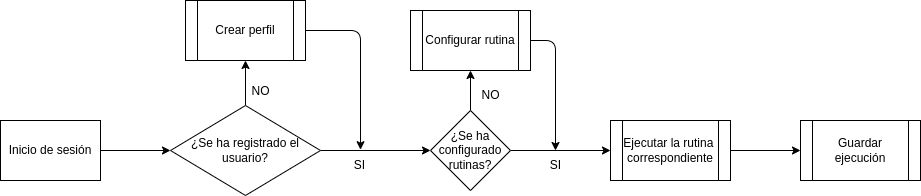
\includegraphics[scale=0.5]{images/diagram-flow.png}
    \caption{Flujo normal asociado a una rutina de entrenamiento}
    \label{fig: diagram-flow}
\end{figure}

Para iniciar el proceso, el usuario debe ingresar sus credenciales en la interfaz de Inicio de Sesión, como se muestra en el Figura \ref{annex: 2}(a). En caso de que el usuario no tenga una cuenta registrada en el sistema, será redirigido automáticamente a la interfaz de registro, (ver Figura \ref{annex: 2}(b)). En este paso, se le permitirá crear un nuevo usuario para poder acceder al sistema. Tras iniciar sesión, se despliega la interfaz principal, brindando al usuario la capacidad de realizar diversas acciones, tales como configurar y dar inicio a un proceso de entrenamiento ( Figura \ref{annex: 3}(a) y \ref{annex: 3}(b)), iniciar el proceso de calibración (Figura \ref{annex: 3}(c)), examinar estadísticas relevantes (Figura \ref{annex: 5}) y revisar o editar la información detallada en su perfil (Figura \ref{annex: 4}a y \ref{annex: 4}(b)) así como elegir una rutina ya configurada (Figura \ref{annex: 4}(c)).

Si la rutina de entrenamiento deseada no se encuentra disponible, el usuario tiene la posibilidad de interactuar directamente con la aplicación accediendo a la interfaz de configuración de parámetros correspondiente a la modalidad que desea establecer. En el caso de la modalidad Ligero, (Figura \ref{annex: 3}a), se le solicita al usuario ingresar manualmente los valores de distancia o tiempo, específicos al nivel de dificultad del entrenamiento que busca. Por otro lado, en la modalidad Clínico (Figura \ref{annex: 3}(b) y \ref{annex: 3}(c)), la interacción se intensifica, ya que el usuario debe calibrar el sistema para obtener los valores esenciales de línea base y MCV. A partir de este último valor, el usuario asume un papel activo al elegir el porcentaje que se asignará a la rutina de rehabilitación por canal, basándose en criterios médicos. Una vez que se han establecido estos parámetros, el usuario continúa su interacción con la aplicación al ingresar los valores específicos de distancia o tiempo correspondientes a la rutina de entrenamiento Clínico.

Al hacer clic en el botón \underline{Comenzar}, se presenta la escena de juego correspondiente a la rutina configurada \ref{annex: 6}. Al finalizar, los resultados obtenidos son almacenados en la base de datos y pueden ser visualizados en la sección de estadísticas de la interfaz. 